\documentclass[conference]{IEEEtran}
\IEEEoverridecommandlockouts
% The preceding line is only needed to identify funding in the first footnote. If that is unneeded, please comment it out.
\usepackage{cite}
\usepackage{lipsum}
\usepackage{amsmath,amssymb,amsfonts}
\usepackage{algorithmic}
\usepackage{graphicx}
\usepackage{hyperref}
\usepackage{pdfpages}
\usepackage{gensymb}
\usepackage{textcomp}
\usepackage{xcolor}
\usepackage{float}
\restylefloat{table}


\hypersetup{
    colorlinks=false, %set true if you want colored links
    linktoc=all,     %set to all if you want both sections and subsections linked
    linkcolor=blue,  %choose some color if you want links to stand out
}

\begin{document}
\bstctlcite{IEEEexample:BSTcontrol}

\title{Convolutional Neural Networks for Super High Momentum Spectrometer Optics Pattern Recognition
%\thanks{Identify applicable funding agency here. If none, delete this.}
}

\author{\IEEEauthorblockN{Zain Mothupi}
\IEEEauthorblockA{\textit{Department of Physics} \\
\textit{University of Warwick}\\
Coventry, England \\
mothupizain@gmail.com}
%\and
%\IEEEauthorblockN{2\textsuperscript{nd} Given Name Surname}
%\IEEEauthorblockA{\textit{dept. name of organization (of Aff.)} \\
%\textit{name of organization (of Aff.)}\\
%City, Country \\
%email address or ORCID}
%\and
%\IEEEauthorblockN{3\textsuperscript{rd} Given Name Surname}
%\IEEEauthorblockA{\textit{dept. name of organization (of Aff.)} \\
%\textit{name of organization (of Aff.)}\\
%City, Country \\
%email address or ORCID}
%\and
%\IEEEauthorblockN{4\textsuperscript{th} Given Name Surname}
%\IEEEauthorblockA{\textit{dept. name of organization (of Aff.)} \\
%\textit{name of organization (of Aff.)}\\
%City, Country \\
%email address or ORCID}
%\and
%\IEEEauthorblockN{5\textsuperscript{th} Given Name Surname}
%\IEEEauthorblockA{\textit{dept. name of organization (of Aff.)} \\
%\textit{name of organization (of Aff.)}\\
%City, Country \\
%email address or ORCID}
%\and
%\IEEEauthorblockN{6\textsuperscript{th} Given Name Surname}
%\IEEEauthorblockA{\textit{dept. name of organization (of Aff.)} \\
%\textit{name of organization (of Aff.)}\\
%City, Country \\
%email address or ORCID}
}



\maketitle

\thispagestyle{plain}
\pagestyle{plain}

\begin{abstract}
Our research focused on developing algorithms for the recognition and prediction of specific tune patterns in spectrometer optics data from Experimantal Hall C at Jefferson Laboratory. The main goal was to create a machine learning model capable of recognizing optics patterns that would otherwise be tedious for humans to classify, in a mere matter of seconds with reasonably high accuracy. Specifically, we utilised the Keras deep learning Application Programming Interface(API) to build a Convolutional Neural Network(CNN). The CNN was trained on a dataset of 186 simulated optics patterns and a Cross-Entropy function was implemented to assess the model's accuracy throughout the training process. The model was able to reach an average accuracy close to 100\text{\%} and an average loss of approximately 0.3. The machine learning model's ability to predict output was then tested against a set of 60 new images and achieved an average accuracy of 83\text{\%}.  
\end{abstract}

%\begin{IEEEkeywords}
% Here you would put keywords that may be important to follow in the paper (maybe repeated terms of importance, e.g. neural networks, convolution, )
%\end{IEEEkeywords}

\section{Introduction}
Since the inception of Artificial Intelligence in the mid 20th century, there has been rapid progress towards the creation of systems capable of matching or even surpassing human ability. As a result, Machine Learning (ML), a subset of artificial intelligence, emerged. In ML computer systems learn to perform tasks without explicit instructions as they learn purely from a set of data. The concept of computers learning directly from data has led to many algorithms modelled after the way humans learn. In particular, Neural Networks were inspired by the wiring of the human brain, imitating the interconnectedness of the neurons.
 See Fig.\ref{fig:Artificial_Neural_Network}


% Here you would insert an image (for example, the cartoon of the neural network brain)
\begin{figure}[htb!]  % you can google what eahc of these options, e.g. [h!] means when placing a picture, and you can adjust accordingly
  \centering
  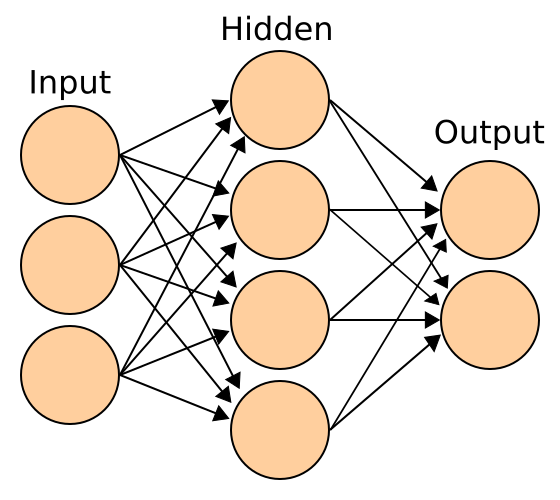
\includegraphics[scale=0.3]{images/Artificial_neural_network.png}
  \caption{Example of an Artificial Neural Network. \\ \centering Note: Reprinted from Ref.\cite{Artificial_Neural_Network}.}
  \label{fig:Artificial_Neural_Network}
\end{figure}

In our research, we used a specific type of Neural Network known as a Convolutional Neural Network to interpret and analyse images. All CNNs follow a basic list of steps in order to learn patterns from data:
\begin{itemize}
\item receive input data
\item make a prediction
\item assess the prediction by comparing it to the desired output
\item adjust its internal structure to give more accurate predictions the next time
\end{itemize}

A simple illustration of a neural network architecture is shown in Fig.\ref{fig:CNN_Image} 
\begin{figure}[h]
 \centering
  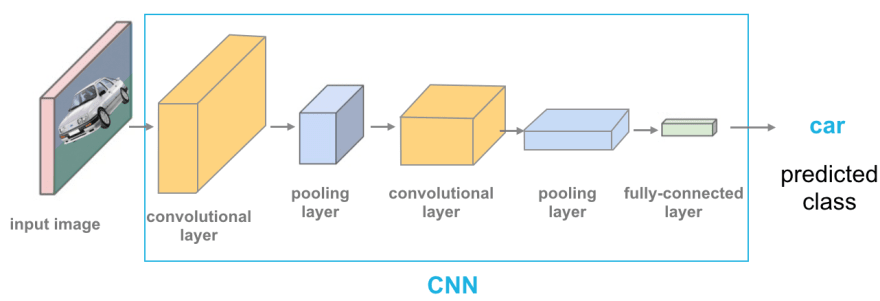
\includegraphics[scale=0.3]{images/ConvolutionalNeuralNetwork.png}
  \caption{Illustration of the structure of a Convolutional Neural Network. \\ \centering Note: Reprinted from Ref.\cite{CNN_Image}.}
  \label{fig:CNN_Image}
\end{figure}



\section{Methodology}
In this research, we analyze a total of 186 distinct simulated optics patterns from the Super High Momentum Spectrometer (SHMS) at Hall C of Jefferson Lab.
There were six different optics correlations ( $x_{fp}$ vs. $y_{fp}$,  $x_{pfp}$ vs. $y_{pfp}$, $x_{fp}$ vs. $y_{pfp}$,  $x_{pfp}$ vs. $y_{fp}$, $x_{fp}$ vs. $x_{pfp}$ and  $y_{pfp}$ vs. $y_{fp}$ . Here the first "fp" refers to the focal plane, which is an imaginary plane in the spectrometer where the transported particles are focused to and the first "p" refers to the prime symbol which is a derivative of the focal plane variable with respect to the opotical z-axis along which particles are transported. Each pattern had 31 optics images with varying optics tunes [Q1, Q2, Q3], corresponding to the spectrometer quadrupole magnets, summarized in Table \ref{tab:tune_stpSize}:

\begin{table}[ht!]
	\begin{center}
		\begin{tabular}{llll} % left-aligned, number of l's represent number of headings
                  \hline
                  Quadrupole Magnet & Range & Stepsize \\
                  \hline\hline
	          $Q1$ & [0.90, 1.10] & 0.02  \\
                  $Q2$ & [0.95, 1.05] & 0.01  \\
                  $Q3$ & [0.90, 1.10] & 0.02  \\                       
                  \hline 
		\end{tabular}
	\end{center}
	\caption{Summary of the variance of Optics tunes during the training process.}
	\label{tab:tune_stpSize}
\end{table}

Each of the six 2D SHMS optics pattern correlations were trained separately, using 31 different optics tunes
per correlation plot for a total of 186 images. The optics patterns for testing the network consisted of only
varying Q2 from 0.945 to 1.055 in steps of 0.01, while keeping Q1 and Q3 tunes fixed at unity.
To test the neural network after it had been trained, a set of 10 images were used for each 2D optics correlation, where Q1 and Q3
tunes were kept fixed at unity while Q2 was varied from 0.955 to 1.055 in steps of 0.01 for a total of 10 Q2 tunes.\\ Figure. \ref{fig:2d_correlation2} shows an example of a 2D Optics Correlation Plot.


\begin{figure}[h]
 \centering
  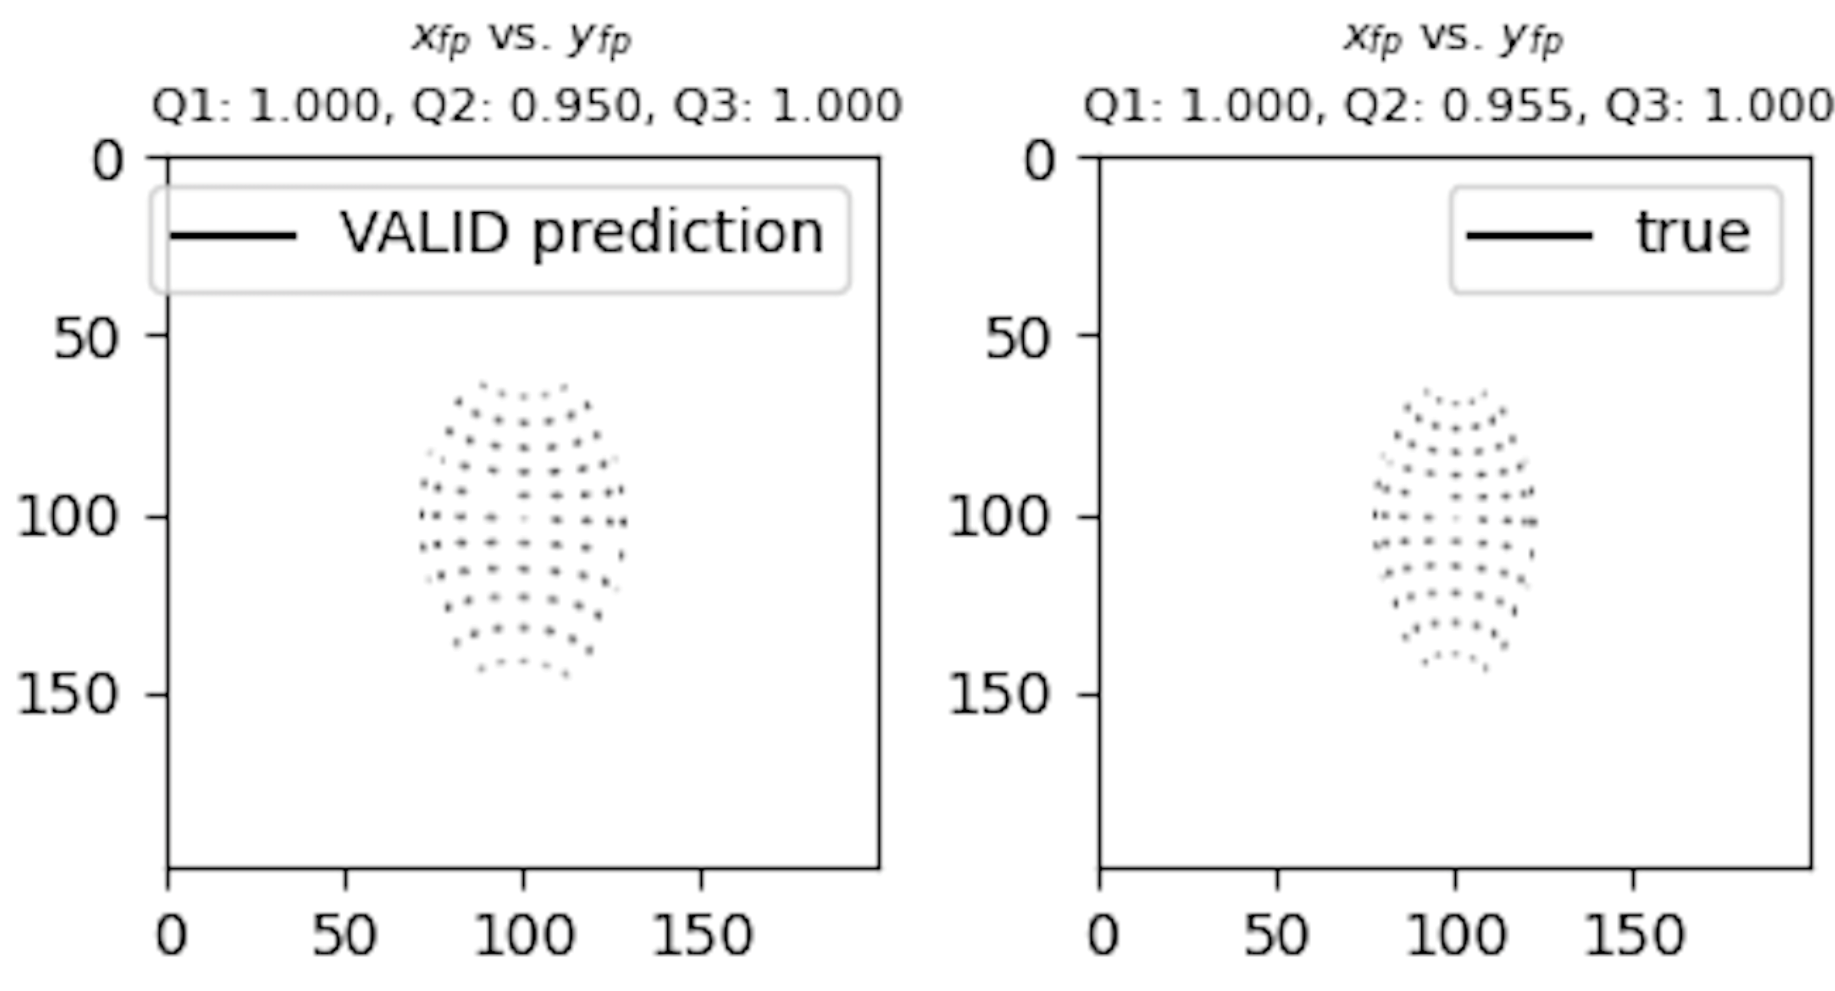
\includegraphics[scale=0.2]{images/2d_correlation2.png}
  \caption{Example of a 2D Optics Correlation with the Predicted(left) and True(right) Optics Patterns.}
  \label{fig:2d_correlation2}
\end{figure}





\section{Data Analysis Procedure}


%This figure position may need to be changed and put someplace else in this file, depending on whether it shows up
%in the location you want in your pdf. (Let me know if you have any issues with the placement of this picture)

\indent Our Neural Network utilised 5 layers in total(See Fig.\ref{fig:CNN_layers}). It consisted of input and output layers which represent the raw input image and output prediction and intermediate hidden layers each with a specific image analysis task. The intermediate layers are the \emph{Convolutional layer, Pooling layer} and \emph{Activation layer} described in the subsections below.\\

\begin{figure}[ht!]
  \centering
  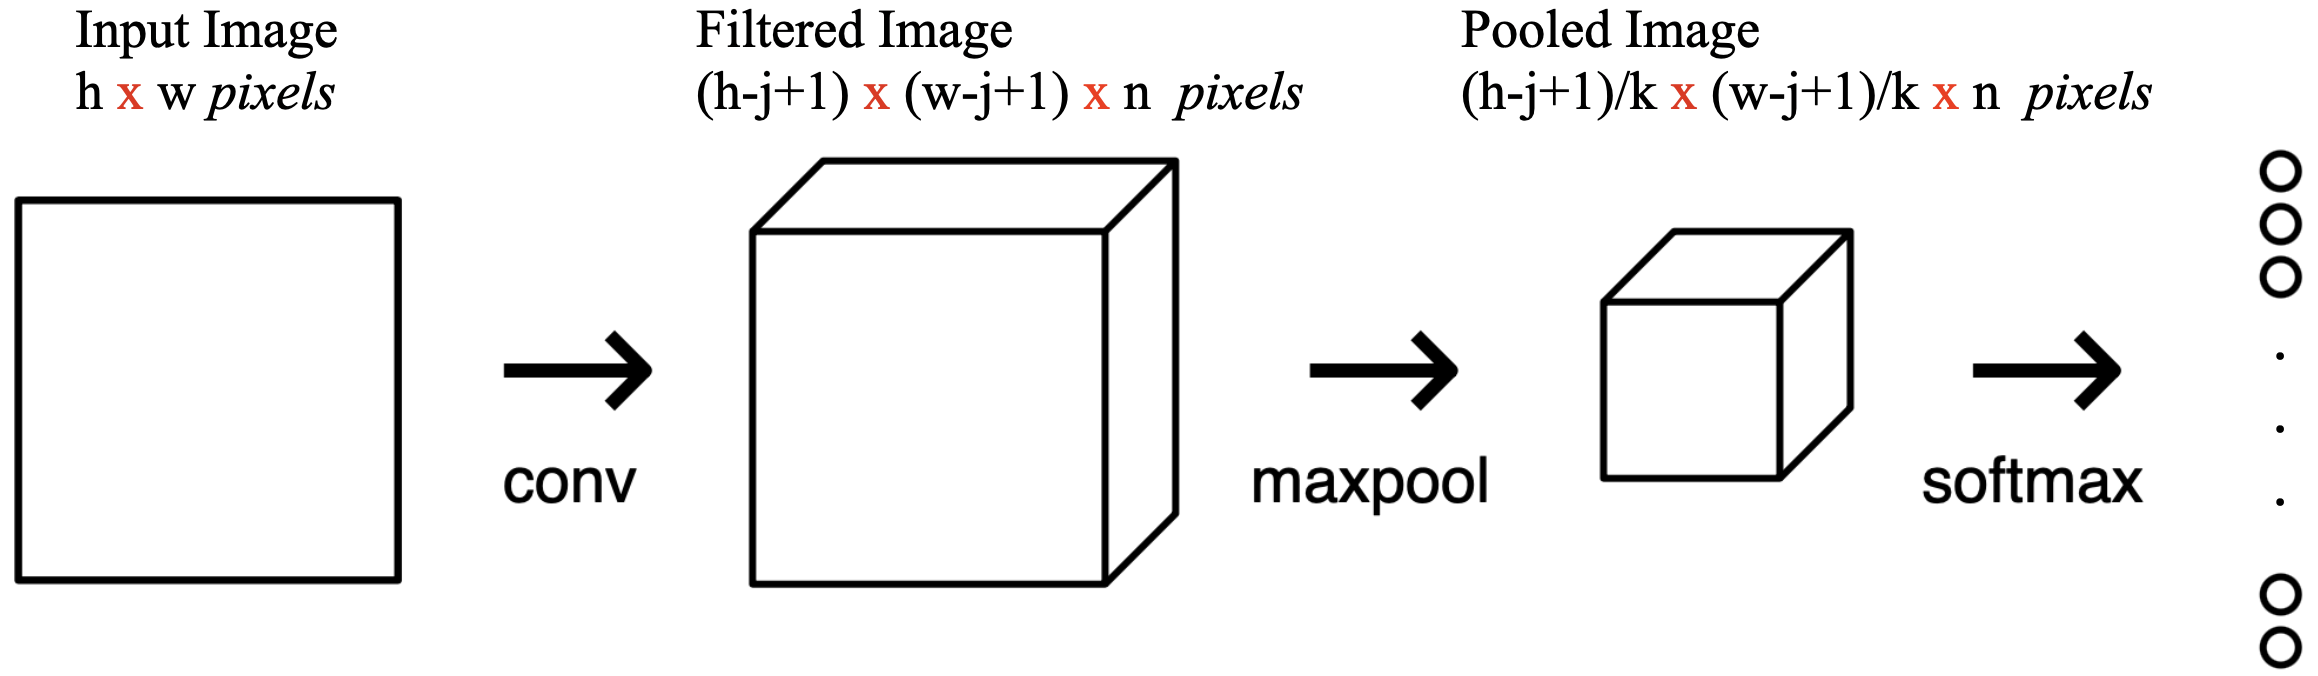
\includegraphics[scale=0.2]{images/CNN_layers.png}
  \caption{Structure of the Convolutional Neural Network used in this analysis.}
  \label{fig:CNN_layers}

\end{figure}

\subsection{Convolutional Layer}
The convolutional layer contains a set of 12 filters with dimension 6x6,  which are convolved with the input image and outputted by the layer. The process of convolving the image with the filters consists of overlaying the filter over a group of pixels (with the same dimensions as the filter), carrying out element-wise multiplication, calculating the sum of the results and using this as a pixel value in the output image. We then move on to the next possible grouping of pixels and continue the process until the entire image has been convolved with the filter. Convolutional layers help detect specific localized features in images which aids the model in making more accurate predictions (see Ref.\cite{CNNPart1_VZ_2019}).
\subsection{Pooling Layer}
We used a pooling size of 6 which decreaseS the size of  our input images from 200x200 to 32x32 pixels. This allows for the model to reduces the number of computations it has to perform while still preserving the important elements of the image. This is achieved by “pooling” or grouping pixel values together and selecting the maximum of the values which acts as a summary of the features present in the region (see Ref.\cite{CNNPart1_VZ_2019}).
\subsection{Activation Layer}
The activation layer uses a function known as an activation function to transform an unbounded input to a bounded output. In this research we used the Softmax function as our activation function. The Softmax function is given by $\text{Softmax}(x_{i}) = \frac{\exp(x_i)}{\sum_j \exp(x_j)}$ and turns the neural network's output values into probabilities which are more useful when evaluating our models predictions as it allows us to assess the certainty with which the NN makes a prediction. We assess the performance of our NN using a loss function. The loss function compares the prediction of the NN to the actual value and calculates how far off the model is. This is then feed back to NN so that it can adjust its weights and biases to achieve a lower loss or higher accuracy (See Ref. \cite{Softmax}).

\subsection{Backpropagation}

The input image is passed through all the layers and the final output of the Softmax layer is a prediction. The prediction is then compared to the known result and the loss is calculated. A backpropagation method is used to minimize the loss by updating the parameters of the NN so as to decrease the loss. Each combination of a forward runthrough of  the NN and updating of parameters via backproagation is known as an epoch. The updated parameters are then analysed through the same process for a certain number of epochs so that the loss is minimized.

\subsection{Data Analysis Procedure}
The data with specific [Q1,Q2,Q3] tunes were simulated using the standard Hall C simulation program (\texttt{mc-single-arm})
and the raw data output was written to a ROOTfile. A separate ROOT C++ script (\texttt{make\_2Doptics.C}) was used to form each of
the six abovementioned 2D focal plane correlations correlations which were stored in a separate ROOTfile as histogram objects.
The 2D histograms were then converted to a 2D pixelated array and stored in binary format (.h5) via a Python code (\texttt{save2binary.py})
array to be read by the Neural Network using Python Keras. Each optics image used was 200x200 pixels and was passed thorugh each of
the hidden layers of the network described in Section 4 of this article.


\section{Results and Discussion}

\indent In this research our aim was to teach a computer to recognize optics patterns that would otherwise be tedious or difficult to distinguish for humans. Using the Keras API we trained and tested a CNN by providing simulated optics data from Jefferson Laboratory, Hall C. Each of the six 2D optics correlations were trained with 31 optics tunes and were able to reach and plateau at an accuracy of 98\% and a loss of 0.3 in 100 epochs. We used 10 test images per optics correlation and the network was able to correctly predict the patterns with at least 83\% accuracy. The results of the training are shown in Fig.\ref{fig:Results_part1} and Fig.\ref{fig:Results_part2}. 

\begin{figure}[ht!]
  \centering
  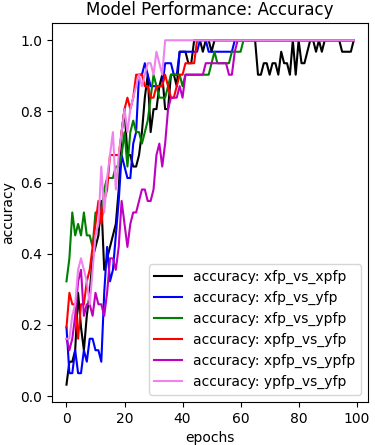
\includegraphics[scale=0.6]{images/Results_part1.png}
  \caption{Plot of Accuracy vs Number of Epochs}
  \label{fig:Results_part1}
\end{figure}

\begin{figure}[ht!]
  \centering
  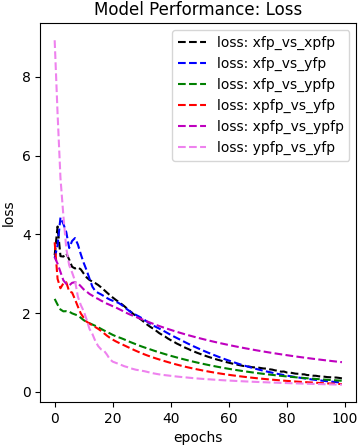
\includegraphics[scale=0.6]{images/Results_part2.png}
  \caption{Plot of Loss vs number of Epochs}
  \label{fig:Results_part2}
\end{figure}

The results of the test images is summarized in Table  \ref{tab:results} where $N_{c}$ represents the number of correctly predicted patterns and $N_{t}$ represents the total number of patterns.
\begin{table}[h]
	\begin{center}
		\begin{tabular}{ p{2cm}p{1cm}p{1cm}p{1cm}  } % left-aligned, number of l's represent number of headings
                  \hline
                  2D Optics \\Correlation  & $N_{c}$  & $N_{t}$ & Accuracy \\ \hline \hline
	          $x_{fp}$ vs. $y_{fp}$ & 9 & 10 &  90\% \\
                   $x_{pfp}$ vs. $y_{pfp}$ & 10 & 10 & 100\%\\
                   $x_{fp}$ vs. $y_{pfp}$ & 10 & 10 & 100\%\\
                   $x_{pfp}$ vs. $y_{fp}$ & 5 & 10 & 50\%\\
                   $x_{fp}$ vs. $x_{pfp}$ & 9 & 10 & 90\%\\
                   $y_{pfp}$ vs. $y_{fp}$ & 7 & 10 & 70\%\\

                  

    
		  \hline 
		\end{tabular}
	\end{center}
	\caption{Performance of the trained CNN for each of the 2D optics correlation patterns.}
	\label{tab:results}
\end{table}




These results show that the computer can achieve a reasonably high accuracy and low loss during training. The test data shows us that when given new data the model still outputs reliable predictions for the majority of optics correlations. However, from these results we can see that the model had trouble predicting the correct labels for the $x_{pfp}$ vs. $y_{fp}$ and  $y_{pfp}$ vs. $y_{fp}$  optics correlations. To improve the predictions we could decrease the step size between the optics tunes so that the neural network can learn to distinguish more subtle features in the data which will allow it to make more accurate predictions. Altogeher we have demonstrated that the model can recognize these optics patterns fairly well and with a few adjustments could be used to support humans in greatly reducing the time taken to classify these optics tune patterns.








%dummy text
%\lipsum

\bibliography{references}   
\bibliographystyle{IEEEtran}



\end{document}
